\section{Frequency analysis of music}
In this section the recordings of music will undergo frequency analysis, and the goal is to be able to express which frequencies the tones played in the recordings are generally found at.
\subsection{Single tones}\label{sec:single}
Firstly, the tuning of guitar is checked for consistency. The low and high E strings on the guitar should vibrate and emit sounds frequencies of 82.41 Hz and 329.63 Hz, respectively. Figures \ref{fig:single_low} and \ref{fig:single_high} show the frequency spectra for the recordings of the two tones.
\begin{figure}[H]
\centering
\begin{subfigure}{0.49\textwidth}
\centering
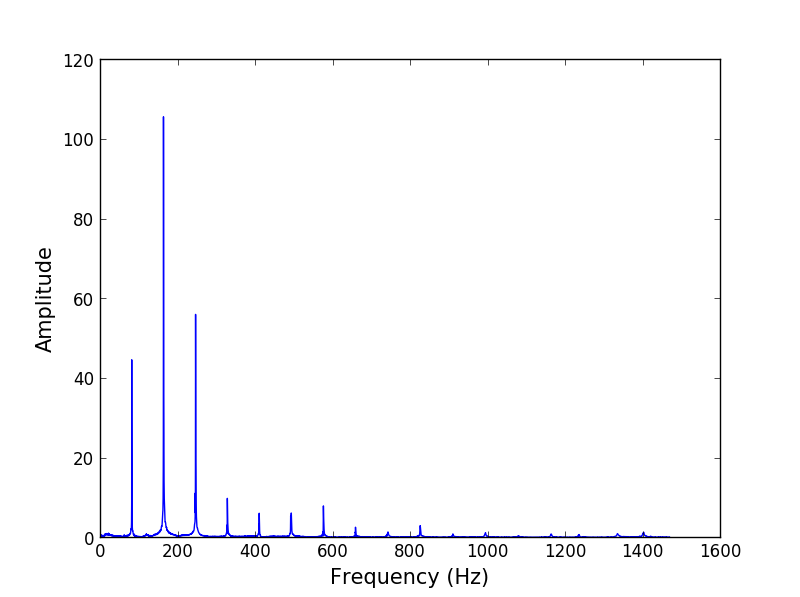
\includegraphics[width=\textwidth]{figures/freqanal/single_low.png}
\caption{Low E string.}
\label{fig:single_low}
\end{subfigure}
\begin{subfigure}{0.49\textwidth}
\centering
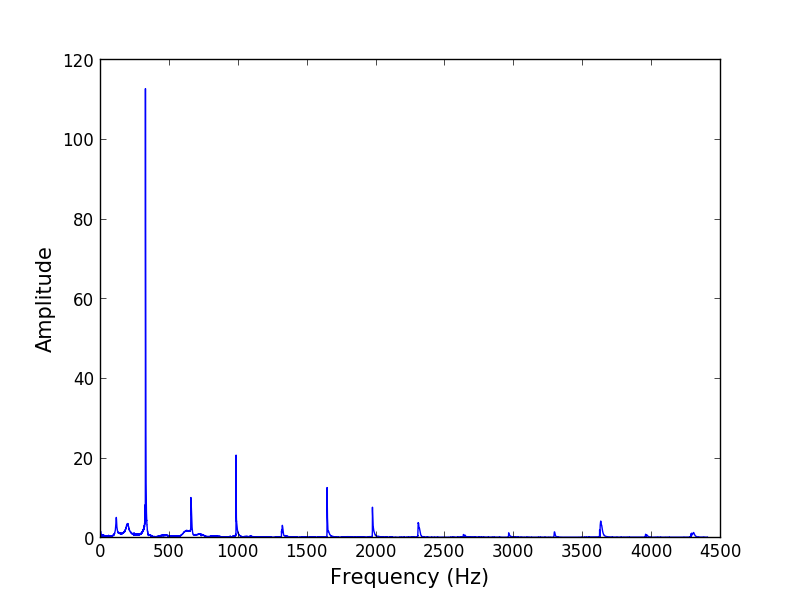
\includegraphics[width=\textwidth]{figures/freqanal/single_high.png}
\caption{High E string.}
\label{fig:single_high}
\end{subfigure}
\caption{Frequency spectra of low and high E strings on a guitar. The harmonics are clearly visible.}
\label{fig:single}
\end{figure}
The most significant frequencies in the two recordings are 163.82 Hz and 329.83 for the low and high E's, respectively. As $163.82$ Hz $\approx 2\cdot82.41$ Hz this is regarded as a harmonic of the low E. The harmonics are moreover observable in the figures as reduced peaks at integer multiples of the fundamental frequencies of the tones. It is furthermore seen from the figures, that the energy in the signals is mainly located at frequencies above 75 Hz and below 1000 Hz for the low E and above 100 Hz and below 2000 Hz for the high E.
\subsection{Chords}
Figures \ref{fig:chord_low} and \ref{fig:chord_high} show the frequency spectra of the recordings of low and high E chords, respectively.
\begin{figure}[H]
\centering
\begin{subfigure}{0.49\textwidth}
\centering
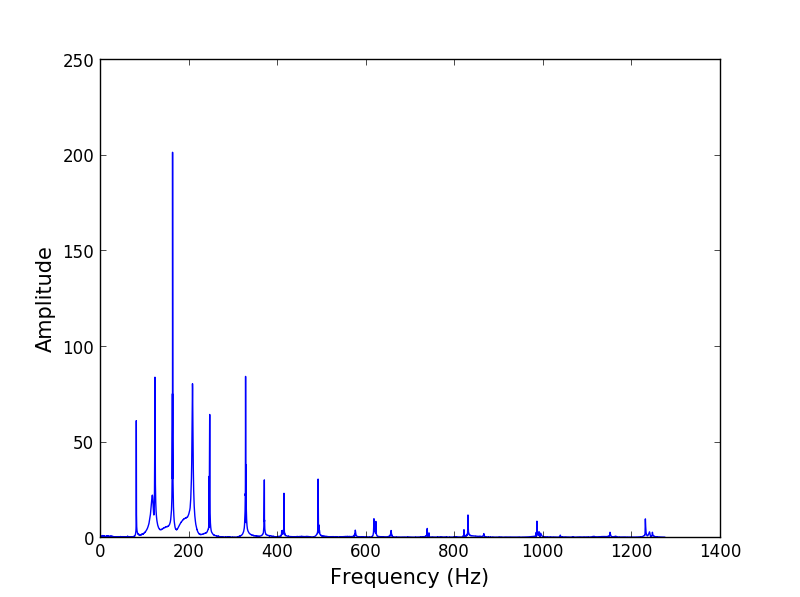
\includegraphics[width=\textwidth]{figures/freqanal/chord_low.png}
\caption{Low E chord.}
\label{fig:chord_low}
\end{subfigure}
\begin{subfigure}{0.49\textwidth}
\centering
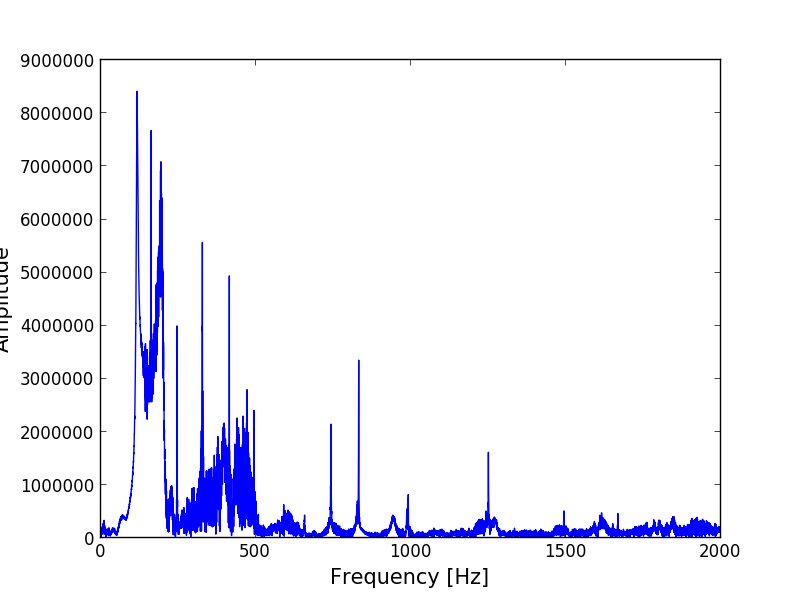
\includegraphics[width = \textwidth]{figures/freqanal/chord_high.png}
\caption{High E chord.}
\label{fig:chord_high}
\end{subfigure}
\caption{Frequency spectra of low and high E chords played on a guitar}
\label{fig:chord}
\end{figure}
The most significant frequencies are 163.86 Hz and 119.27 Hz. Once again it is assumed that the higher frequency of the low pitch E is due to harmonics. These frequencies do furthermore not correspond to a specific note - this is assumed to be because of the composition of chords being of multiple tones. The majority of the energy in the signals is located above 80 Hz and below 1000 Hz.
\subsection{Scale}
Figure \ref{fig:scale_fast} shows the frequency spectrum of playing a octatonic scale.
\begin{figure}[H]
\centering
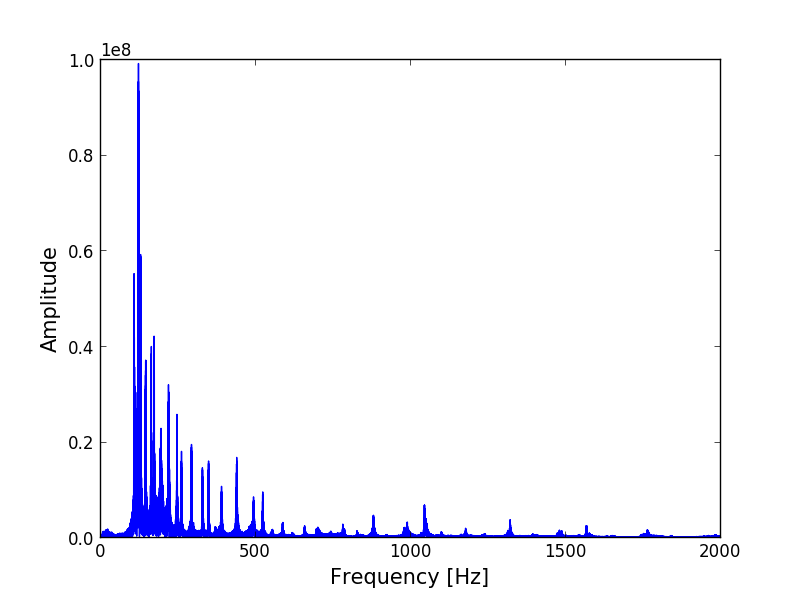
\includegraphics[width=0.7\textwidth]{figures/freqanal/scale_fast.png}
\caption{Frequency spectrum of an octatonic scale played quickly.}
\label{fig:scale_fast}
\end{figure}
The majority of the energy in the signal is as seen located above 100 Hz and below 600 Hz.

\subsection{Melody with single notes}
Figures \ref{fig:melody_single} show the frequency spectrum for a melody consisting only of single tones played slowly.
\begin{figure}[H]
\centering
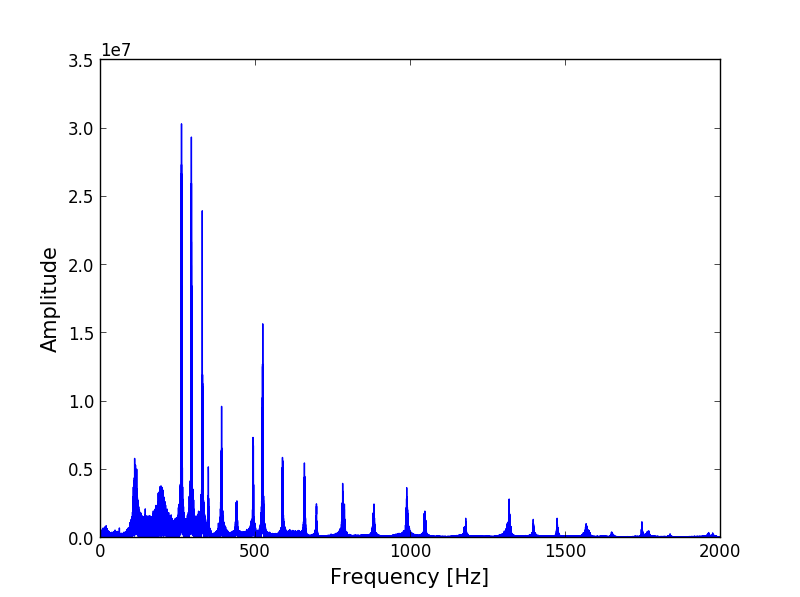
\includegraphics[width=0.7\textwidth]{figures/freqanal/melody_single.png}
\caption{Frequency spectrum of Itsy Bitsy Spider played on a guitar with only singe strings plucked.}
\label{fig:melody_single}
\end{figure}
The majority of energy in the signal is located above 100 Hz and below 2000 Hz.
\subsection{Melody with chords}
In figures \ref{fig:melody_chords} is seen the frequency spectrum for a melody consisting of chords played slowly.
\begin{figure}[H]
\centering
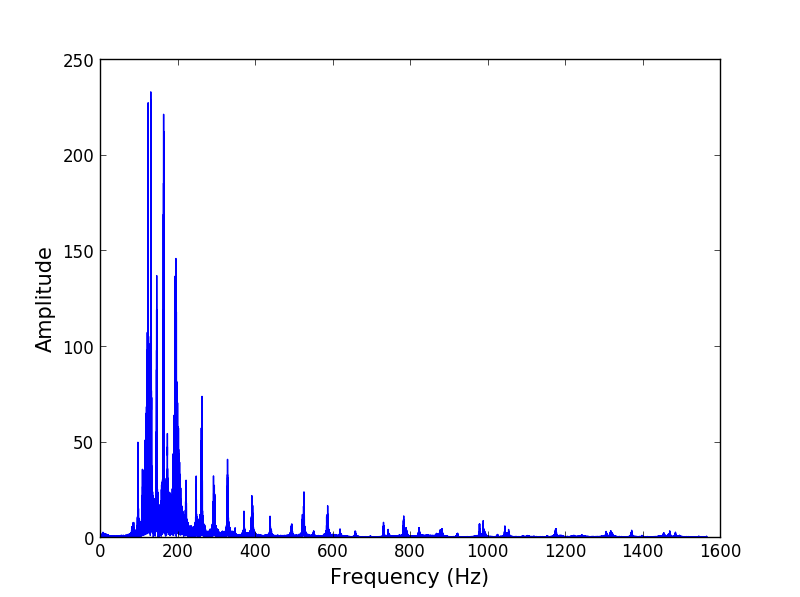
\includegraphics[width=0.7\textwidth]{figures/freqanal/melody_chords.png}
\caption{Frequency spectrum of melody played with chords.}
\label{fig:melody_chords}
\end{figure}
The majority of energy in the signal is located above 90 Hz and below 800 Hz.

\section{Frequency analysis of noise}
In this section the recordings of noise will undergo frequency analysis, and the goal is to be able to express which frequencies the recorded noise is generally found at.
\subsection{Folding paper and clapping}
Figure \ref{fig:clapping} and \ref{fig:folding} show the frequency spectrum of clapping at equidistant intervals in time and folding a piece of paper, respectively.
\begin{figure}[H]
\centering
\begin{subfigure}{0.49\textwidth}
\centering
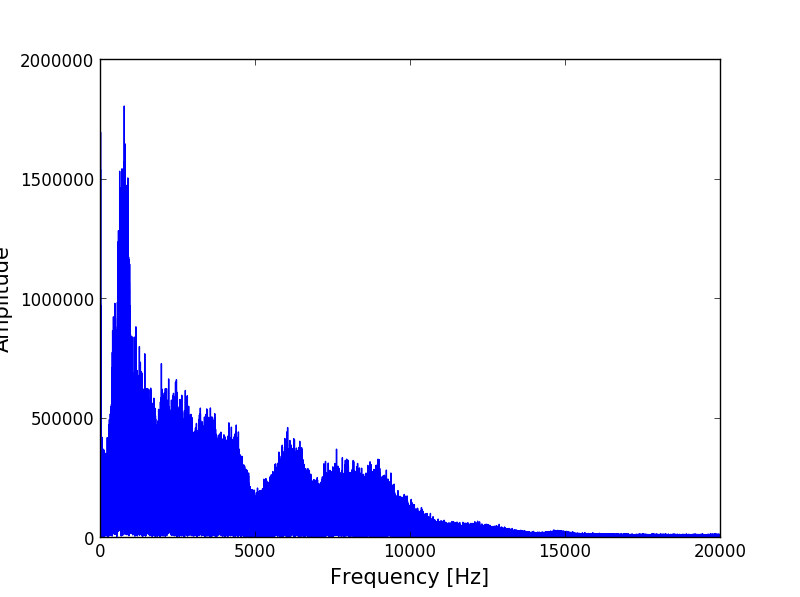
\includegraphics[width=\textwidth]{figures/freqanal/clapping.png}
\caption{Clapping}
\label{fig:clapping}
\end{subfigure}
\begin{subfigure}{0.49\textwidth}
\centering
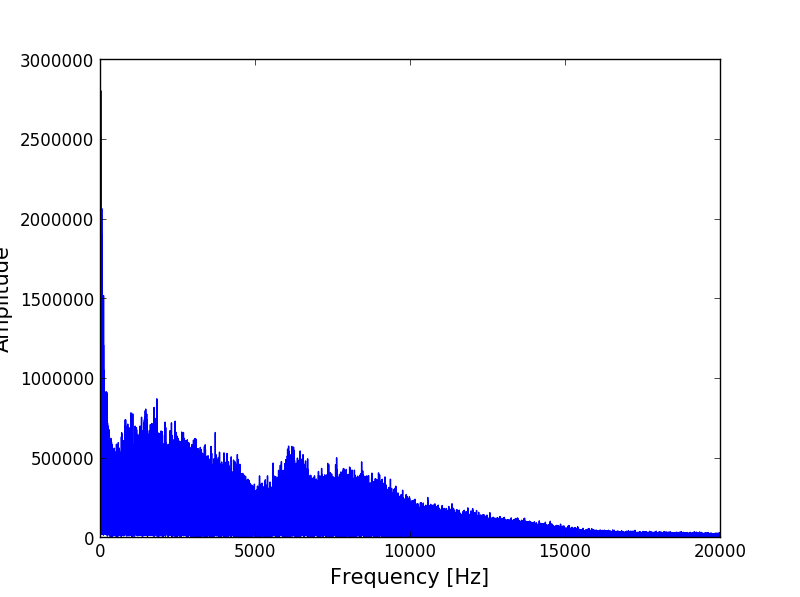
\includegraphics[width=\textwidth]{figures/freqanal/folding.png}
\caption{Folding a piece of paper}
\label{fig:folding}
\end{subfigure}
\caption{Frequency spectra of different noises.}
\end{figure}
The majority of the energy in both noises is located between 0 and 15000 Hz.
\subsection{Singing and talking}
Figures \ref{fig:talk} and \ref{fig:song} show the frequency spectrum of recorded talking and singing respectively.
\begin{figure}[H]
\centering
\begin{subfigure}{0.49\textwidth}
\centering
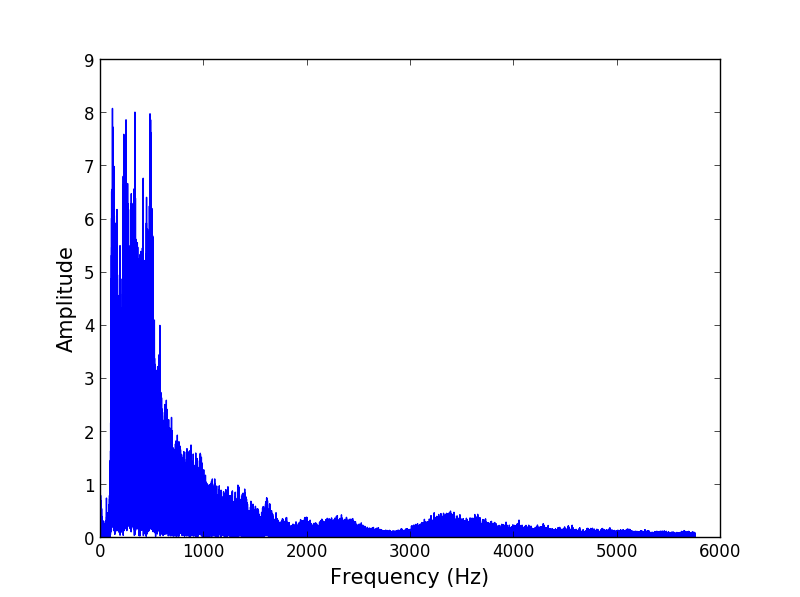
\includegraphics[width=\textwidth]{figures/freqanal/talk.png}
\caption{Person talking}
\label{fig:talk}
\end{subfigure}
\begin{subfigure}{0.49\textwidth}
\centering
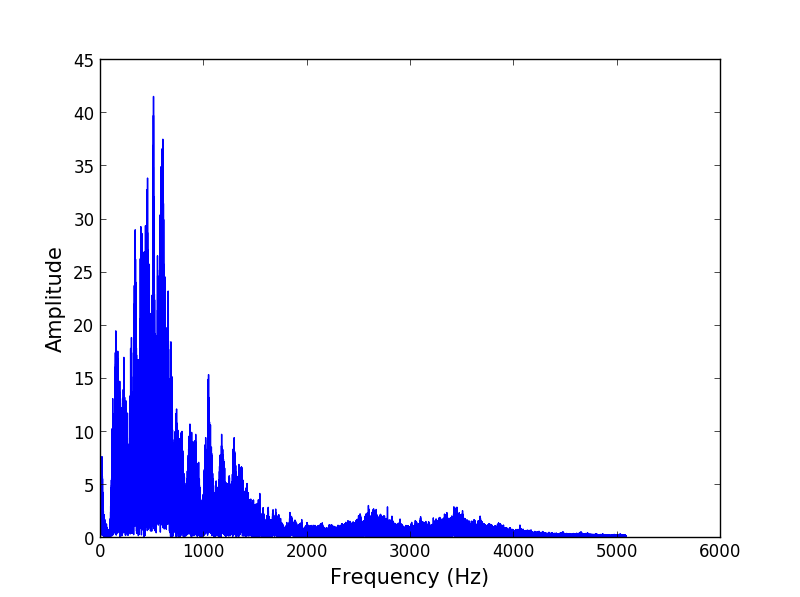
\includegraphics[width=\textwidth]{figures/freqanal/song.png}
\caption{Person singing}
\label{fig:song}
\end{subfigure}
\caption{Frequency spectra of a person talking and signing.}
\end{figure}
The majority of the energy is located between 100 and 5000 Hz for talking and 0 and 5000 Hz for singing.
\subsection{Ambient noise}
Figure \ref{fig:ambient} shows the frequency spectrum of the abient noise recorded in a parking lot at the campus of AAU.
\begin{figure}[H]
\centering
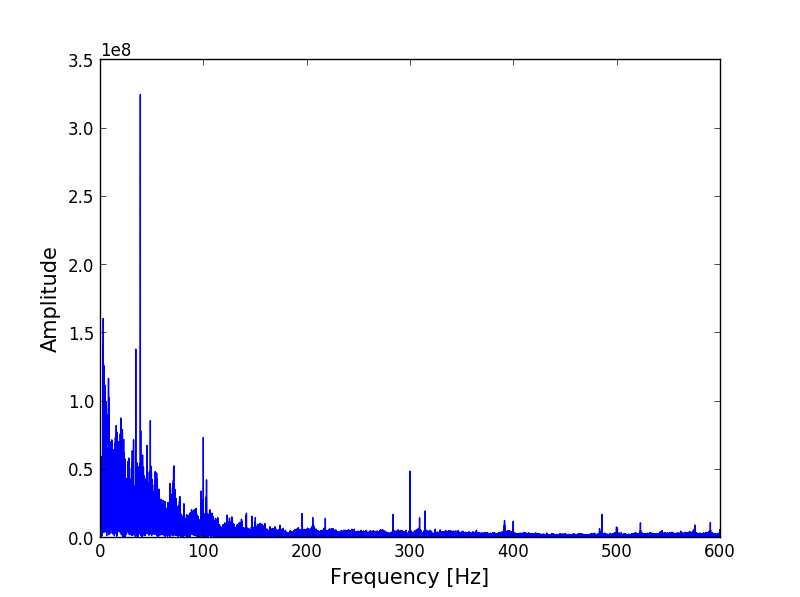
\includegraphics[width=0.7\textwidth]{figures/freqanal/ambient.png}
\caption{Frequency spectrum for ambient sound.}
\label{fig:ambient}
\end{figure}
The majority of the energy in the signal is located between 0 and 600 Hz.











